\section*{Electricity and Magnetism Highlights}
\addcontentsline{toc}{section}{\protect\numberline{}Electricity and Magnetism Highlights}
Some of my personal favorite electricity and magnetism problems. These are hard problems, but I strongly encourage you to give most of these a try (except problem 1), because they're good problems. If you feel like you've attempted a problem several times and come up with an incorrect answer, I'd be happy to discuss these with you and go over them.\\
\textbf{Problems:}\\
1. (?? $\bigstar$) Find as many mistakes/inaccuracies as you can in the Electricity and Magnetism section. \\
2. (3 $\bigstar$) A uniformly charged nonconducting solid sphere of radius $a$ has its center at the origin and has a uniform volume charge density of $\rho$. Material is removed from the sphere leaving a spherical cavity that has a radius $r < \frac{a}{2}$ and its center at $x=b$ ($b< \frac{a}{2}$) on the $x$-axis. Show that the electric field inside the cavity is uniform, directed in the $+x$-direction, and has magnitude $\frac{\rho b}{3\epsilon_0}$. \\
3. (3 $\bigstar$, $\spadesuit$) A non-conducting disk has radius $R$, carries a uniform surface charge density $\sigma$, and rotates with angular speed $\omega$. a) Consider an annular strip that has a radius $r$, a width $dr$, and a charge $dq$. Show that the current $dI$ produced by this rotating strip is given by $\sigma \omega r\, dr$. b) Use your result from part a) to show that the magnetic field strength at the center of the disk is given by the expression $B = \frac{1}{2} \mu_0 \sigma \omega R$. c) Use part a) again to show that the magnetic field strength at a point on the central axis of the disk a distance $z$ from its center is $B = \frac{1}{2} \mu_0 \sigma \omega \left(\frac{R^2 + 2z^2}{\sqrt{R^2 + z^2}} - 2z\right)$.\\
4. (4 $\bigstar$) A wooden cylinder with mass $m$, radius $R$, and length $L$ has $N$ turns of wire wrapped around it longitudinally so that the plane of the wire coil contains the long central axis of the cylinder. The cylinder is released on a plane inclined at an angle $\theta$ to the horizontal, with the plane of the coil parallel to the inclined plane. If there is a vertical uniform magnetic field of magnitude $B$, show that the least current $I$ through the coil that keeps the cylinder from rolling down the plane is $\frac{mg}{2NLB}$.\\
5. (5 $\bigstar$, $\spadesuit$) In the circuit shown in the figure below, switch $S$ has been open for a long time. At time $t = 0$ the switch is then closed.
\begin{center}
	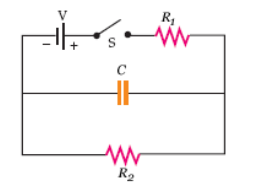
\includegraphics[scale=1]{images/em/RC-problem3.png}
\end{center}
Show that the charge on the capacitor in the steady state is $Q = \frac{\mathscr{E}CR_2}{R_1+R_2}$, and that the charge of the capacitor as a function of time is $\frac{\mathscr{E}CR_2}{R_1+R_2}(1- e^{-\frac{t}{CR_1R_2/(R_1+R_2)}})$.\\
6. (5 $\bigstar$, $\spadesuit$) Consider the circuit shown in the figure where the inductor has negligible
internal resistance and the switch S has been open for a long time. The switch is then closed at time $t=0$.
\begin{center}
	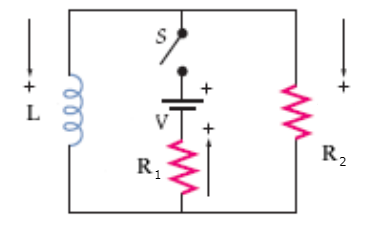
\includegraphics[scale=0.5]{images/em/LR-problem1.png}
\end{center}
Show that the current in the resistor $R_2$ approaches zero in the steady state, and that the current in this resistor can be modeled as $I_2 = \frac{\mathscr{E}}{R_1+R_2}e^{-t(R_1+R_2)/LR_1R_2}$.\\
7. (4 $\bigstar$, $\spadesuit$) A long straight conducting wire with radius $R$ carries a non-uniform current density of magnitude $j(r) = j_0\frac{r}{R}$, where $j_0$ is a positive constant and $r$ is the distance from the axis of symmetry of the wire. This variability in current density is achieved by constructing the wire from a material with variable conductivity $\sigma(r) = \sigma_0 \frac{r}{R}$, where $\sigma_0$ is a positive constant. Let $I$ be the total current in the wire. a) Show that $j_0 = \frac{3I}{2\pi R^2}$. b) Show that if $r>R$, the magnitude of the magnetic field is $B = \frac{\mu_0 I}{2\pi r}$, and if $r < R$, the magnitude of the magnetic field is $B = \frac{\mu_0 I r^2}{2\pi R^3}$. c) Show that the resistance of such a wire with length $L$ is $R = \frac{3L}{\sigma_02\pi R^2}$.\\
8. (4 $\bigstar$, $\spadesuit$) One final railgun problem. A rigid metal bar of length $L$ and mass $m$ slides on two fixed parallel horizontal conducting rods. The bar slides with negligible air resistance and friction. The bar and rods have negligible resistance and form a complete circuit with a sizable resistor of resistance $R$. The system is immersed in a uniform vertical magnetic field of strength $B$. Starting from rest at time $t=0$, the bar is pulled horizontally away from the resistor by an applied constant horizontal force of magnitude $F_0$. Once the bar is in motion, an induced current flows in the bar, and after some time the bar nears a terminal speed $v_T$. a) Show that the terminal speed $v_T = \frac{F_0R}{L^2B^2}$. b) Show that the time it takes for the speed of the bar to reach 3/5 of its terminal speed is $t = \frac{mR}{L^2B^2} \ln \frac{5}{2}$.

\pagebreak